\section{Introduction to Model building}

\subsection*{Definition}
 Model building is the process that allows getting the atomic interpretation of an electron density map. Although a electron density volume can be obtained from different methodologies, in this tutorial we focus in maps obtained by cryo-EM. As an example of these maps, \ffigure{fig:model_building_example} shows the input electron density map (a), as well as the output haemoglobin tetramer atomic model (b) obtained by the model building process. Since high quality atomic structures are essential to accomplish detailed mechanistic studies and to seek inhibitor drugs of macromolecules, the main aim of model building is obtaining reliable structures of these macromolecules. 
 

\begin{figure}[H]
 \centering
 \captionsetup{width=.8\linewidth}  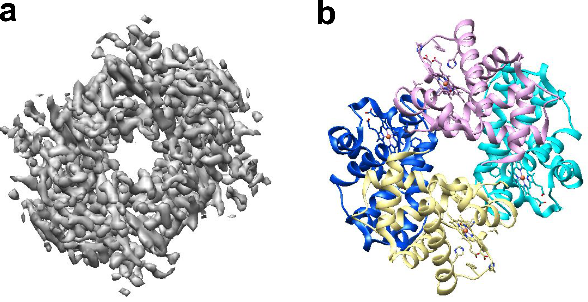
\includegraphics[width=0.6\textwidth]
  {{Images/Fig1.pdf}}
  \caption{Haemoglobin tetramer \citep{khoshouei2017}. a) Electron density map at 3.2\AA\ resolution obtained by Cryo-EM single particle analysis with Volta phase plate. b) Atomic structure model inferred from the electron density volume.}
  \label{fig:model_building_example}
  \end{figure} 
 

\subsection*{Relevance of cryo-EM map resolution}

Model building process is limited by the resolution of the starting cryo-EM density map. The higher the resolution, the more detailed and reliable atomic structure will be obtained. Fortunately, single-particle cryo-EM is undergoing in this decade a resolution revolution that has allowed the structures of macromolecules to be solved at near-atomic resolution. The density map is thus sufficiently resolved to build the atomic model. As a general rule, at resolutions of 4.5\AA\ the molecule backbone can be inferred based on the map alone, and resolutions lower than 4\AA\ allow to trace side chains of some residues. 

 \subsection*{ Model building workflow}
 
 The set of successive tasks aimed to get the atomic interpretation of electron density maps is known as model building workflow. Main steps of the general workflow are detailed from top to bottom in \ffigure{fig:model_building_workflow}. Tasks and tools required are highlighted in green (left side). Before starting those tasks, a detailed study and recruiting of experimental information of the macromolecule itself and similar specimens is recommended. Cryo-EM density map preprocessing is also desirable in order to optimize it by maximizing details and connectivity, as well as extracting the lower asymmetrical element of the starting volume (AU: asymmetric unit) to save computational resources and facilitate the modeling.
 
 In addition to the map AU, the workflow considers as input the sequence of each individual structural element (from 1 to n). This sequence is used to get the initial model, \iii{de novo} or by prediction based in structures of homologous sequences. Initial model of each structure element has to be fitted to the volume AU, and then refined according to the density of this map fraction. Refinement in real and/or reciprocal spaces are included in the workflow. Once refined, the geometry of each individual structure has to be validated regarding the starting volume. The last two steps of refinement and validation will be applied globally to the whole set of structures contained in that map AU to avoid forbidden steric overlaps among them. Borders between adjacent unit cells will be checked similarly in the reconstruction of the whole atomic structure. 
 
 In this tutorial, we show how to obtain an atomic model using a reference homologous structure.
 
% of model building every step of the general workflow will be considered, except the $de novo$ modeling step because the appropriate tools to accomplish this type of modeling are not still implemented in \scipion. 
 
\begin{figure}[H]
 \centering
 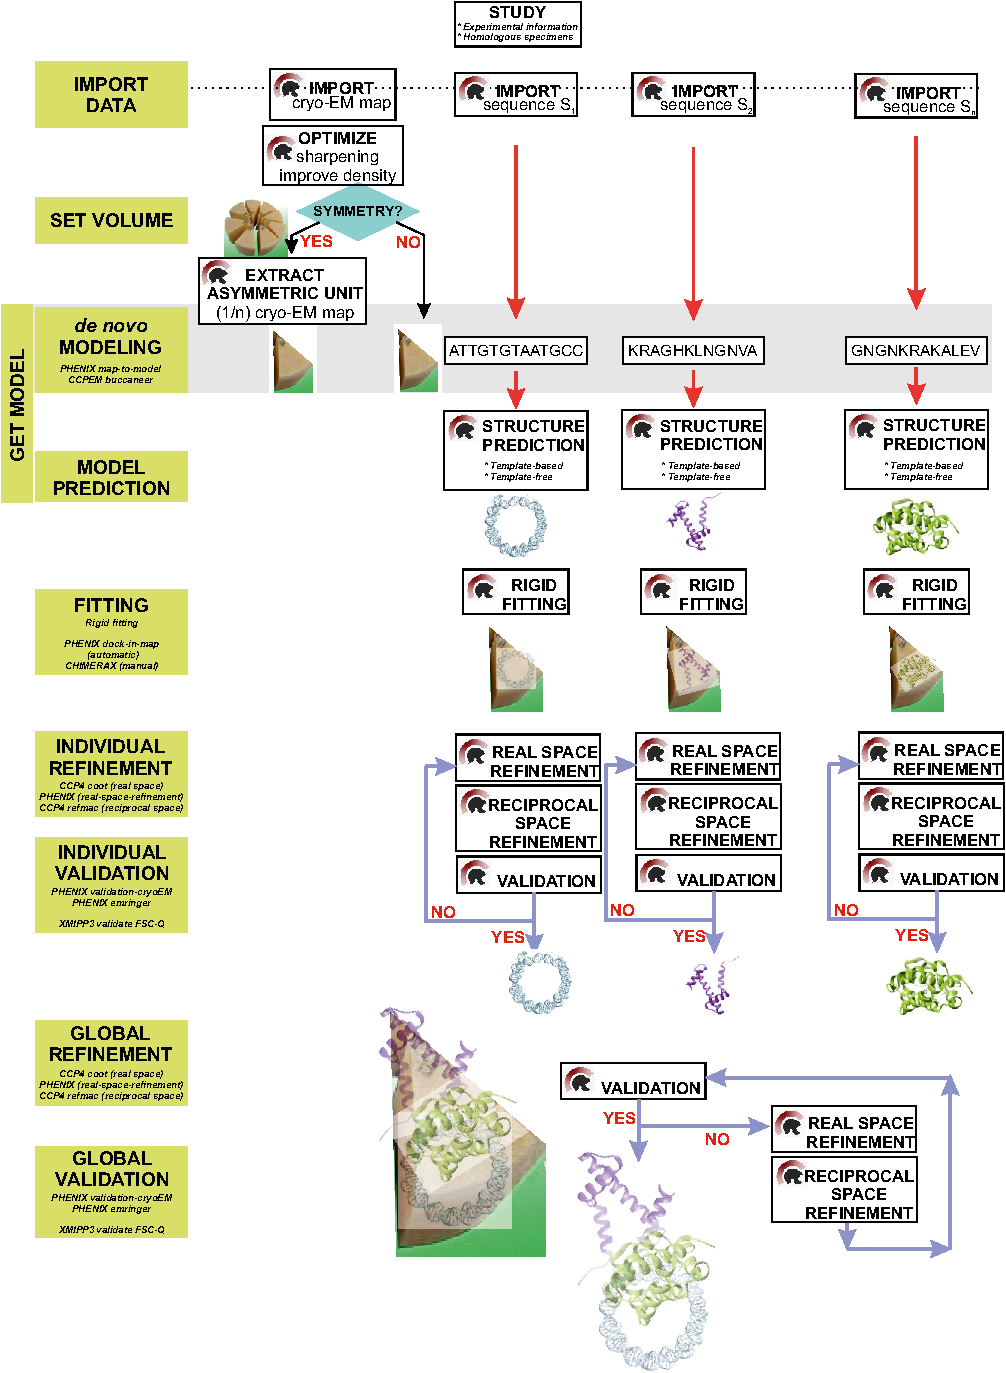
\includegraphics[width=0.95\textwidth]
  {{Images/Fig2.pdf}}
  \caption{General Model Building Workflow.}
  \label{fig:model_building_workflow}
  \end{figure} 
  
